\chapter{GLOBAL MOTOR INVARIANT}
\label{chap:gi}


\nomenclature[a1]{$q$}{Generalized Coordinates}
\nomenclature[a2]{$\qd$}{Generalized Velocity}
\nomenclature[a3]{$\state$}{State Variable}
\nomenclature[a4]{$u$}{Control Input}
\nomenclature[a5]{$\mathrm{g}$}{Gravity}

\nomenclature[b1]{$Q$}{Configuration Space or Configuration Manifold}
\nomenclature[b2]{$TQ$}{Tangent Bundle of $Q$}
\nomenclature[b3]{$M$}{State Space Manifold}
\nomenclature[b4]{$TM$}{Tangent Bundle Manifold}



\nomenclature[c1]{$\mathcal{A}$}{Attractor}
\nomenclature[c2]{$\mathcal{Boa}(\mathcal{A})$}{Basin of Attraction of $\mathcal{A}$}
\nomenclature[c3]{$\simeq$}{Topology Conjungacy}



\nomenclature[d1]{$S$}{Neural Oscillator}
\nomenclature[d2]{$\uin$}{Input Signal to the Neural Oscillator}
\nomenclature[d3]{$\uout$}{Output of the Neural Oscillator}
\nomenclature[d4]{$\hin$}{Input Coefficient of the Neural Oscillator}
\nomenclature[d5]{$\hout$}{Output Coefficient of the Neural Oscillator}



%\nomenclature[zcif]{$CIF$}{Cauchy's Integral Formula}                                % first letter Z is for Acronyms 
%\nomenclature[aF]{$F$}{complex function}                                                   % first letter A is for Roman symbols
%\nomenclature[gp]{$\pi$}{ $\simeq 3.14\ldots$}                                             % first letter G is for Greek Symbols
%\nomenclature[gi]{$\iota$}{unit imaginary number $\sqrt{-1}$}                      % first letter G is for Greek Symbols
%\nomenclature[gg]{$\gamma$}{a simply closed curve on a complex plane}  % first letter G is for Greek Symbols
%\nomenclature[xi]{$\oint_\gamma$}{integration around a curve $\gamma$} % first letter X is for Other Symbols
%\nomenclature[rj]{$j$}{superscript index}                                                       % first letter R is for superscripts
%\nomenclature[s0]{$0$}{subscript index}                                                        % first letter S is for subscripts




\graphicspath{{GlobalInvariant/GlobalInvariantFigs/EPS/}{GlobalInvariant/GlobalInvariantFigs/}}


Motions are similar but vary greatly.
For example, different people will walk with different gaits. 
An interesting question  is how the word ``walk'' refers to different gaits.
Motor Invariant Theory(\moit) proposes an answer:  despite differences in gaits, we agree on the word ``walk''  because in essence, we all walk in the same manner.
Intuitively, the gaits are periodic, energy efficient and stable.
The variations come from the differences in body, environment or purpose.
From dynamic perspective, all the gaits dynamics share the same structure, or the qualitative properties of walking are invariant.
In \moit, the qualitative invariant properties are \emph{Global Motor Invariant}.


For the biological perspective, we believe the walking ability is inborn and encoded in the body structure.
What ``Walk'' means is one motion primitive.
In \moit, the motion primitives are identified by the global motor invariant.
This claim will be justified in Section~\ref{sec:GMIandMA}.


In theory, it is difficult to define the gait similarity mathematically.
Topology is introduced for a clear definition of global invariant.
Such a definition has important dynamic meaning, topologically equivalent means that the dynamic systems are qualitatively the same.
Basic ideas of topology and qualitative dynamics are introduced in Section \ref{sec:qualiDy}.

Entrainment is the biologically based method to maintain the global motor invariant.
We will discuss the theory and experiments in Sections~\ref{sec:cpgcontrol} and Section~\ref{sec:qualyexample}.







\section{Introduction to Qualitative Dynamics}
\label{sec:qualiDy}
Motion Primitives are ``trivial'' motion tasks.
The evolution process equips animals with a body structure that suits many motion tasks.
As a result,such motion tasks can be accomplished by exploring the natural dynamics without too much control effort.
For the dynamic perspective, the delicate design of body structure permits several patterns when animals interact with the living environment.  
Such patterns exists across detailed variations in body structure such as the tall and short characters and environment like rough or plane ground.
They are robust or \emph{structural stable} in the dynamic term.
In \moit, the identification of motion primitives and adaptation are based on the structural stability.
This section serves as a short introduction to concepts and prepared mathematics.


Qualitative dynamic properties are analysed with the tool of differential topology.
This idea can be traced back to Poincare\citep{Poincar'e1899,Poincar'e1885} and was recently developed by the Smale School\citep{Smale1970}.
There is no enough space to include the whole subject, please refer to book \citep{abraham1978foundations}for more details.
Throughout this thesis,  geometrical perspective is adopted for it is more intuitive.
Some primary knowledge of topology and manifold is required which can be found in ~\citep{abraham1978foundations}.
For the sake of completeness, this thesis will provide a rough and intuitive explanation below.
Intuitive speaking,   \emph{topology} is studies the geometry properties  that are preserved through continuous  deformations, such as twistings and stretchings of objects. Discontinuous deformations like tearing will break the topology. 
Due to this reason, in the topological space, a circle is topologically equivalent to an ellipse because stretching a circle can deform it into an ellipse and a sphere is equivalent to an ellipsoid.
 
A \emph{manifold} is a topological space that  locally looks like the Euclidean space of a specific dimension. 
A line and a circle are one-dimensional manifolds, a plane and sphere  are two-dimensional manifolds, and so on into high-dimensional space.


A dynamic system is usually described as a differential equation, from the geometrical perspective, the differential equation also describes a differentiable manifold.
Qualitative properties can be obtained by analysing the topological  property of geometry.
\emph{Global Motor Invariants} are identified by the topological structure.





\subsection{Dynamic Systems and Differentiable Manifold}
Motions of a mechanical system are determined by its configuration  $q$ in configuration space $Q$ and generalized speed $\qd$ in the tangent space $T_{q}Q$. 
Define the state value $\state=[q,\qd] \in M$, where $M$ is the state space, or state manifold.
A motion is a trajectory $t \mapsto q(t)$ in the configuration space parameterized by time~$t$.
For a dynamic system, $q(t)$ usually is derived from the state trajectory $\state(t)$, which is described by a differential equation. 



For every point $\state \in M$, 
$F$ and $u$ determine a derivative vector $\dot{\state}$ in the \emph{Tangent Space}~$T_{\state}M$. 
Vectors over the full space of $\state$ form the \emph{vector field} $\mathbf{V}$, described by Equation~\ref{eq:ode}.

\begin{equation}
\label{eq:ode}
\dot{\state}=F_{\alpha}(\state)+u
\end{equation}



where $u$ is the control effort, 
$\alpha$ is the system parameters,
and $F$ is determined by the system's natural property.
If $u=0$,  no control effort is applied.
Such systems are \emph{autonomous systems}. 

A solutions to Equation~\ref{eq:ode} is an \emph{integral curve}. 
\emph{Flow} $\Phi(\state)$ of $\mathbf{V}$ is the \emph{integral curve} through~$\state$. 
Flows are usually visualized by a \emph{phase plot}.
All the flows make up the \emph{phase portrait}, which illustrates all the possible motions of the dynamic system.


\textbf{Example}

For a mass-spring system, state variable~$\state=[q,\qd]$ is defined, and Equation~\ref{eq:mass-spring} can be transformed into  Equation~\ref{eq:stateform}.
\begin{equation}
\label{eq:stateform}
\dot{\state}=
\left[ 
\begin{array}{cc}
0 &1\\
-1 &0 
\end{array}
\right]\state
\end{equation}



\subsection{Basin of Attraction}
Intersections of flows are \emph{equilibria}.
At each \textbf{equilibria}, the local space can be divided into subspaces: 
\emph{centre manifold}, \emph{stable manifold}, and \emph{unstable manifold}.
\begin{description} 
\item[centre manifold]
For a flow $\phi_c$ passing through a point $\state_{c}$ on centre sub manifold $W_{c}$, $\phi_c$ will remain on the Centre Manifold. 
\[
\phi_{c}(t) \in W_{c}, t \in R
\]

\item [stable manifold]
For a flow $\phi_{s}$ passing through a point $\state_{s}$ on stable sub manifold $W_{s}$, $\phi_s$ will finally converge to a flow $\phi_c$ on centre manifold.
\[
\phi_{s}(+\infty)=\phi_{c}
\]
\item[unstable manifold]
For a flow $\phi_u$ passing through a point $\state_u$ on unstable manifold $W_{u}$, $\phi_u$ will be repelled from  $\phi_c$ on centre manifold, the inverse of $\phi_u$ converges to $\phi_c$. 
\[
\phi_{u}(-\infty)=\phi_{c}
\] 
\end{description}


\textbf{Attractors} are the equilibria where the whole local space is stable, or the dimension of unstable manifold is zero.
\textbf{Repellors} are the equilibria where the whole local space is unstable, or the dimension of stable manifold is zero.







In theory, only the attractors of the dynamic systems can be  observed  and are of interest in motor control:
\begin{enumerate}
 \item Fixed Point or equilibrium point, a phase plot  is show in Figure~\ref{fig:StablePosture}.
 \item Limit Cycle, a phase plot is shown in Figure~\ref{fig:ecycle}.
 The attractor of a limit cycle has the shape of a cycle, which implies self sustained oscillations or periodic behaviours.
 An attractive limit cycle will attract the neighbouring flows spirals into it over the time.
 Such  a system is stable, if any perturbation move the state off the limit cycle, the system will return to the limit cycle automatically.
 
\end{enumerate}

\begin{figure}
	\begin{center}
	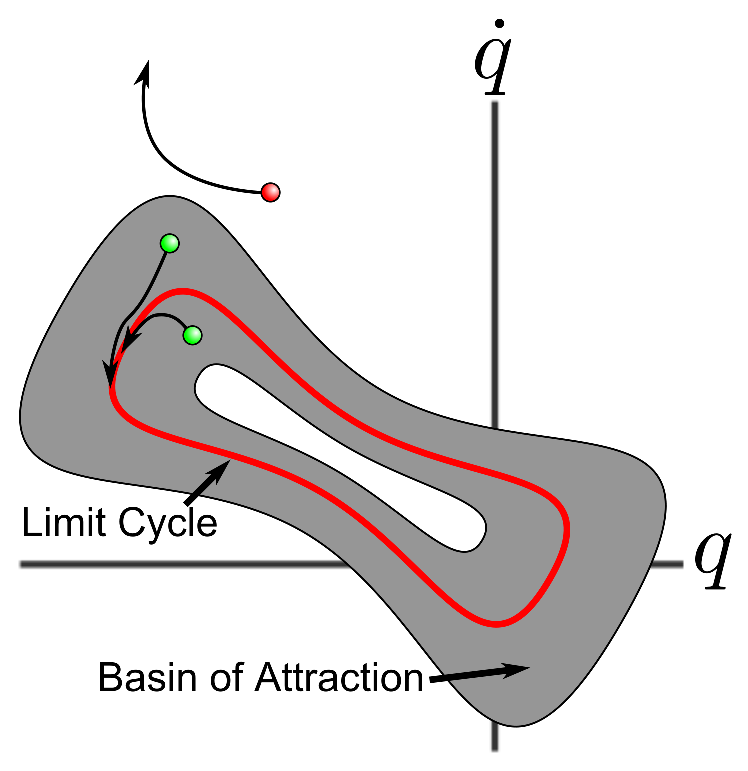
\includegraphics[width=0.5\textwidth]{phase_plot}
	\end{center}
	\caption{Limit Cycle}
	\label{fig:ecycle}
\end{figure}





For non-linear dynamic systems, there may exist many attractors.
The phase plane is divided into different regions,resulting in a cellular structure.
Within each region, all the flows converge to one attractor ~$\mathcal{A}$,
and the corresponding region is  the \emph{basin of attraction} ~$\mathcal{Boa}(\mathcal{A})$.
Figure~\ref{fig:manyboa} shows the landscape of phase portrait of a dynamic system, in which the basins of attraction are coloured differently.
\begin{figure}
\begin{center}
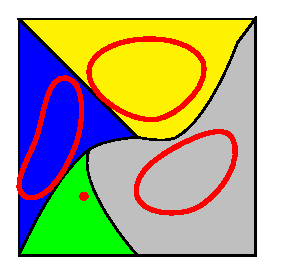
\includegraphics[width=0.4\textwidth]{CellBoa}
\end{center}
\caption{Cellular Structure of Phase Space}
\label{fig:manyboa}
\end{figure}




\subsection{Topological Conjugacy}
The topological structure of a dynamic system can be described by the type of equilibria and the connectivity of their basins of attraction.
Many dynamic systems share the topology structure.
For example, the Duffin system described by Equation ~\ref{eq:duffin} is different from the mass-spring system.
\begin{equation}
\label{eq:duffin}
\ddot{q}+q+q^{3}=0
\end{equation}

However, the two systems share the same topology. 
Phase plots of the two systems are shown in Figure~\ref{fig:msphaseplot} and Figure~\ref{fig:duffin}.
Flows of the two systems are similar, and we can ``deform '' one into another.
This equivalent relationship is  \emph{topological conjugacy}.


\begin{figure}[h]
\begin{center}
	\subfigure[Mass Spring System]
	{
	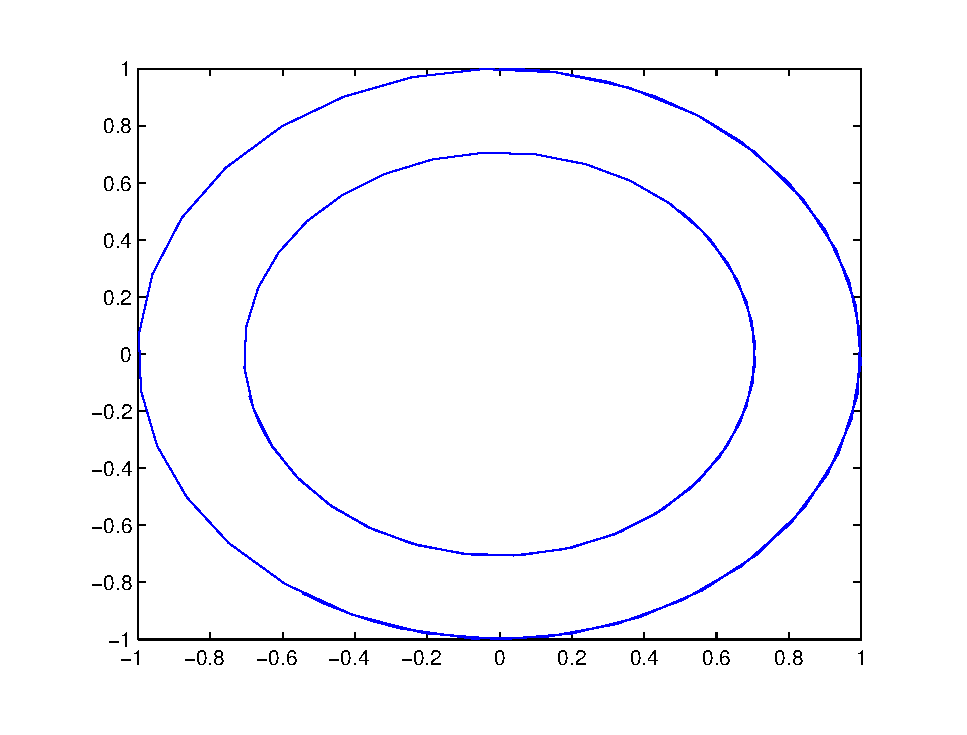
\includegraphics[width=0.45\textwidth]{massspring}
	\label{fig:msphaseplot}
	}
	\subfigure[Duffin System]
	{
	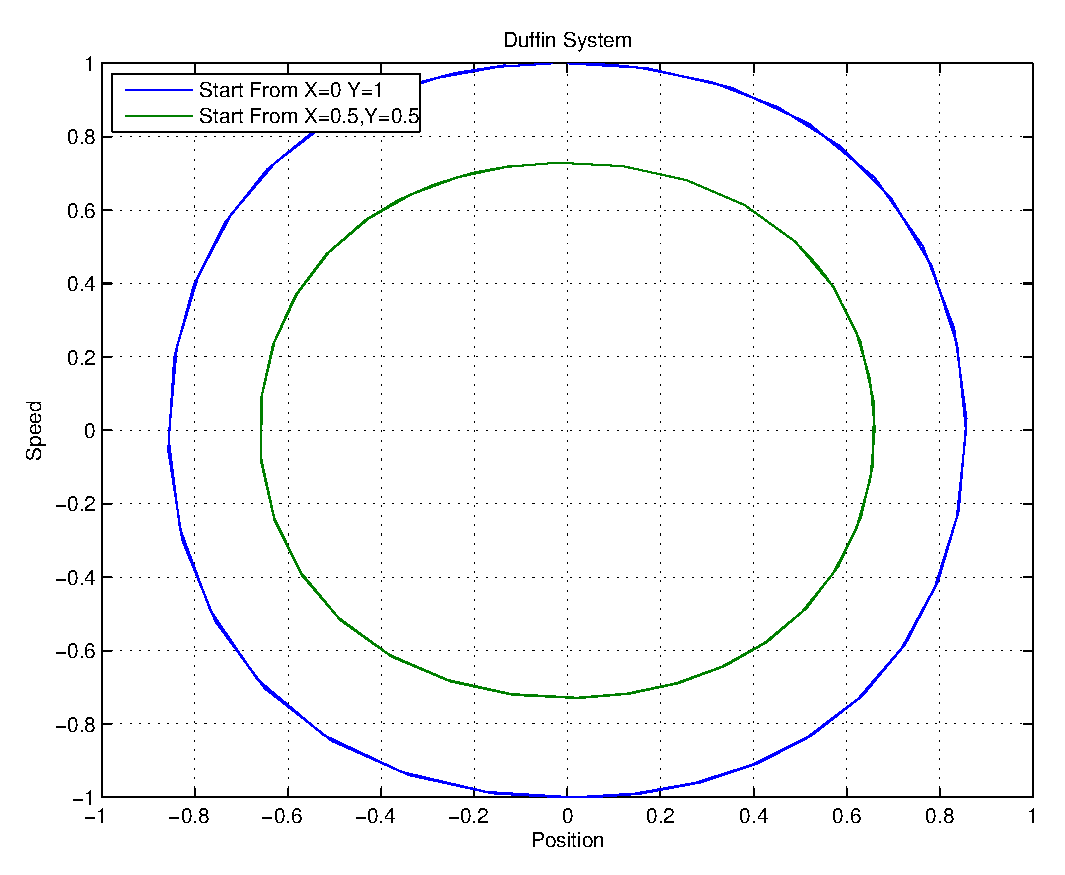
\includegraphics[width=0.45\textwidth]{duffin}
	\label{fig:duffin}
	}	
\end{center}
\caption{Topological Conjugacy}
\label{fig:topconju}
\end{figure}



\begin{mydef}
Let $M$ and $M'$ be topological spaces, and let $F\colon M\to M$ and $F'\colon M'\to M'$
be continuous functions. We say that $F$ is
\emph{topologically conjugate} to $F'$, if there exists a continuous
one-one continuous and invertible mapping $h \colon M\to M'$ such that $h(F(M))=F'(h(M))$.
$h$ is a \emph{topological conjugation} between $F$ and $F'$.
if two systems are topological conjugate, they are \emph{analogous systems}.
\end{mydef}




\section{Global Motor Invariant and Motion Adaptation}
\label{sec:GMIandMA}
Qualitative  dynamic properties are determined by the attractors and its basin of attraction.
\moit\  establishes the relationship between motion primitives and dynamic theory.
In \moit, each attractor and its basin of attraction define a motion primitive.
 `` triviality'' of primitive tasks relies on the attraction.
If the attractor is a fixed point, then the motion will be terminated.
If the attractor is a limit cycle, then the motion will be periodic.
Larger basin of attraction means motion is more stable, while narrow basin of attractions means the fragile stability.
Qualitative property is the \emph{Global Motor Invariant}

\begin{mydef}
\emph{Global Motor Invariant} is the tuple of attractor and its basin of attraction
\end{mydef}


Motions vary because of different perturbations.
In \moit, perturbations are classified in two categories and treated with different control strategies.

\begin{itemize}
\HiItem{State perturbation}

Perturbations that only affect the state $\state$ are \emph{State Perturbations}.
State Perturbations change the current state, but not the underlying dynamic system.


If the perturbed state $\state'$ remains in the basin of attraction, the perturbed flow will converge to the same attractor. 
For the walking example, state perturbations can model the push and recovery motion.
Such a kind of motion adaptation is \emph{Responsive adaptation}.


To make the character more responsive without motion failure,
The motion controller should enlarge the basin of attraction.






\HiItem{Structure Perturbation}
Structure Perturbations affect the dynamic system.
For biological systems,  such perturbations are very common, when a man puts a heavy box on his shoulder or has been injured, the walking dynamic will change due to the structural perturbations.


For some dynamic systems, structural perturbations only deform the phase portrait and result in an analogous system.
This will result in motions variations but qualitative invariant. This kind of motion adaptation is called \emph{system adaptation}.
For \cms, `` motion retargeting'' can be seen as an example of system adaptation.

In some cases, topological structure may not be maintained.
Some perturbations will result in \emph{bifurcation} that violates the topology of the underlying dynamic system.
Such an  example is that the damping perturbations on the mass spring system will change the dynamics qualitatively.
As show in Figure~\ref{fig:dampmass}, damping changes the topology the periodic flows into a fixed point attractor.

\begin{figure}
\begin{center}
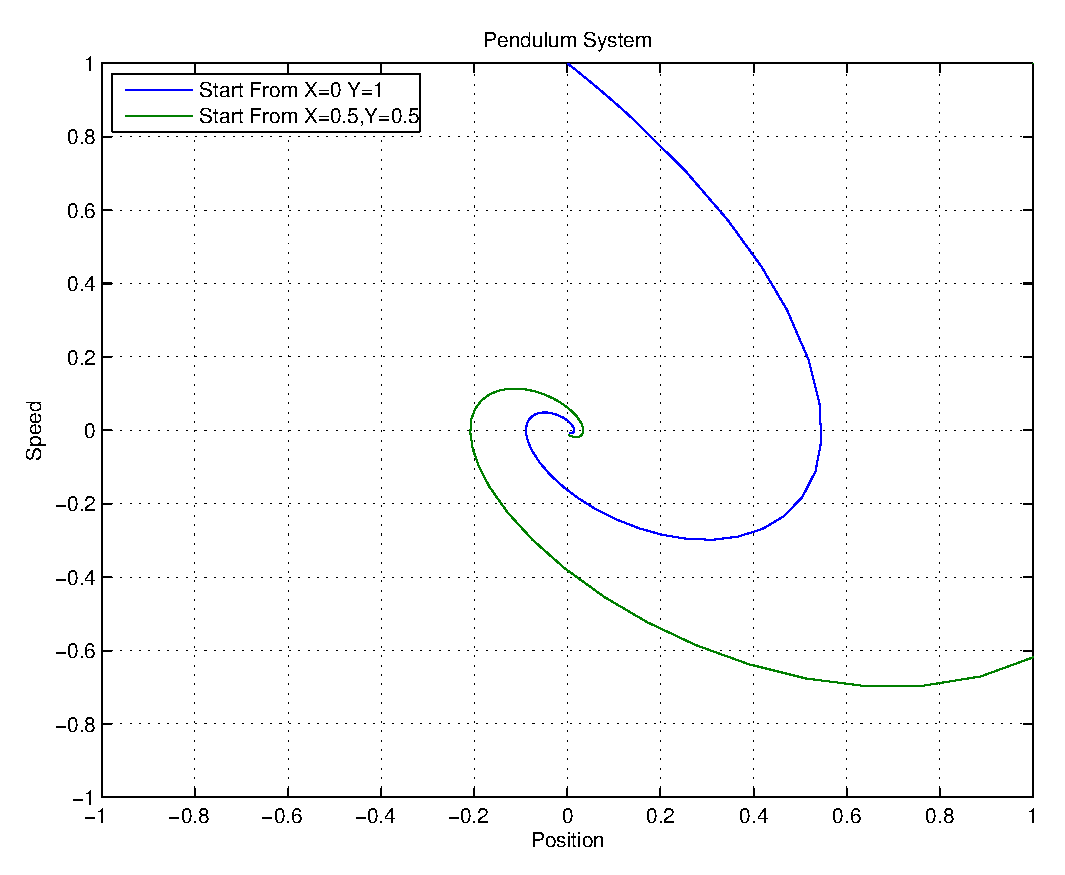
\includegraphics[width=0.5\textwidth]{spring_damping}
\end{center}
\caption{damping perturbation on mass spring system}
\label{fig:dampmass}
\end{figure}

The ability of a dynamic system maintaining its topology structure is \emph{structural stability}.
To make motions adaptive to environment and body changes, controller should boost the structural stability of the motion and prevent bifurcations.
\end{itemize}

These ideas can be seen as a different mathematical interpretation of biological research principles.
For the  \umh,  the basin of attraction of an motion primitive can serve as the uncontrolled manifold of \umh.
State Perturbations are not controlled and motion is freely influenced.
For \eph, attractor of motion primitive is a generalization of equilibrium points.
Impedance control can be seen as adjusting the basin of attraction.





\subsection{Biological Meaning of Structural Stability}
For \cms\ research, Structural Stability is a new idea , but there are good reasons behind it. 
In natural environment, perturbations and uncertainty are everywhere. 
Because of the sensing and computation limitations,  feedback idea  can't cope with all types of perturbations.
In \moit, the alternative idea is such perturbations can be neglected.
If the motion primitive is structural stable, even without control effort, motion and the underlying dynamics will not change qualitatively.
Such an idea can reduce much of the computational burden and provide a framework for motion adaptation.


For biological research questions, the structural stability idea and the qualitative perspective provide better explanations than optimization and feedback theory.

The first is the control difficulty and  evolution of swimming and walking.
From the quantitative perspective, the swimming dynamics are more difficult and walking should be easier.
But from the biological perspective, swimming seems easier, for many primitive life forms exist in water.
The qualitative perspective implies an answer, fluid is continuous and uniform, the dynamics is of simple topological structure and stability is easier to control.
Therefore, fish can maintain its posture with little neural control.
However, on the other side, although the rigid body dynamics for walking are quantitatively easier, the topological structure of walking dynamics is much more complex. 
On the phase plane, there exist many equilibria, and the basin of attraction of walking primitive has limited area,
thus the  stability of walking is fragile and needs more complex measures to enhance.

\moit\ also implies the similarity of the motion style for fish and whales.
In spite of their different position on evolution chain, animals that move through similar environment in a similar manner usually develop similar body structure.
The similarity in body structure promises the same dynamic topology, and motion dynamics are qualitative equivalent.
Also it reminded us that the motion primitive is closely related to the environment, and it is meaningless to talk about walking when the character floating on water, even with the same control strategy, body and environment cannot form the dynamics with desired topological structure.



Further \moit\ suggests the direction of evolution.
For one motion primitive, body may evolve to make the primitive more structural stable.






\section{Global Motor Invariant Control}
\label{sec:cpgcontrol}

In real-life,  natural dynamics can be extremely complex. 
The corresponding manifolds have a complex topological structure, which provides many motion primitives.
For \cms\ applications, the question arises whether different motion primitives can be controlled with a simple and unified method.
The idea is that even there are many motion primitives, attractors can be catalogued in very limited number of types. 
Also even the dimension of dynamic system is large, the dimension of the attractors is not. 
\begin{itemize}
\item Fix point is of zero dimension. 
\item Limit cycle is of one dimension.
\end{itemize}



It is  still under hot debate which type of attractor serves as the foundations for motor control\citep{Degallier2010}.
The current idea is that limit cycle is necessary, based on limit cycle and the fix point can be achieved by
\begin{enumerate} 
\item terminate a limit cycle. 
\item approximated by a limit cycle with small amplitude.
\item Bifurcation. 
\end{enumerate}


Current only the limit cycle is considered in \moit, mainly due to the following two reasons:
\begin{itemize}
\HiItem {periodic behaviour is common} 
Besides the periodic motions such as swimming and running, other biological activities like heart beating, waking and sleeping  are periodic.
A periodic system has the potential to simulate more types of motion and integrate with other biological simulation.

\HiItem{similar results} 
For animations, periodic motions look similar to the terminated motion when the amplitude of limit cycle is small. 
If the oscillation amplitude can be controlled, both types of motion trajectories can be synthesized within one framework.
\end{itemize}

Control strategies are designed based on the type of attractor.
For the fix point attractors, traditional \pd\ controllers are simple and efficient.
For the limit cycle attractors,  entrainment controllers are  proposed as an efficient method.


\subsection{Neural Oscillator and its Stability}


\subsection{\cpg\ and Entrainment}
Biology research suggested that motions are mainly controlled by the organ called \emph{Central Pattern Generator}.
\cpg\ is a small autonomous network that generates rhythmic signals.
From the dynamic perspective, the idea of controlling motion by rhythmic signals can be modelled as entrainment \citep{Gonz'alez-Miranda2004}.
For the situation where two oscillation systems are coupled together, entrainment happens when two systems oscillate in synchronization.
When coupling two oscillation system together, entrainment happens when two systems oscillate in synchronize. 
This effect is also known as a resonant which will enhance the oscillating behaviour. 


For the neural system, it is difficult to carry out precise computation, building an oscillation network is trivial. 
Only two neurons are needed with mutual inhibitive property, as shown in Figure~\ref{fig:cpgdia}.
\begin{figure}[h]
\begin{center}
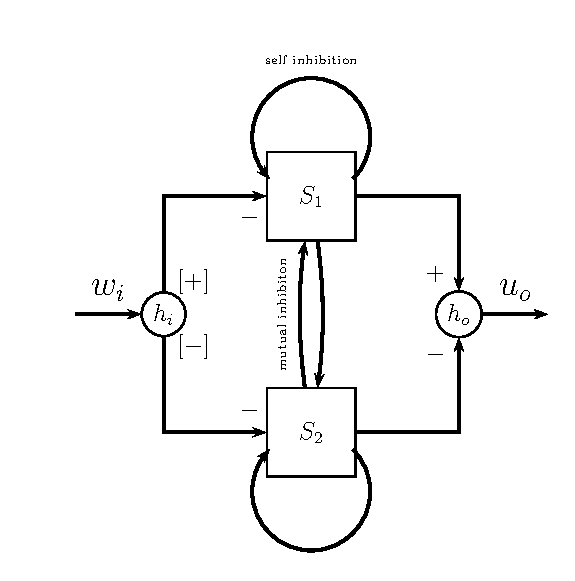
\includegraphics[width=0.4\textwidth]{CPGDiagram}
\caption{Neural Oscillator Structure}
\label{fig:cpgdia}
\end{center}
\end{figure}


One oscillation model was developed  by \citet{neurooscillation} and was extensively studied later on. 
This model can be described as Equation~\ref{eq:matsuta}.

\begin{align}
\tau_{1} \dot{s}_{1}&=c_1-s_{1}-c_2 l_{1}-c_3 [s_{2}]^{+}-\sum_{j}h_{ij}[w_{j}]^{+} \nonumber\\
\tau_{2} \dot{l}_{1}&=[s_{1}]^{+}-l_{1} \nonumber\\
\tau_{1} \dot{s}_{2}&=c_1-s_{2}-c_2 l_{2}-c_3 [s_{1}]^{-}-\sum_{j}h_{ij}[w_{j}]^{-} \nonumber\\
\tau_{2} \dot{l}_{2}&=[s_{2}]^{+}-l_{2}
\label{eq:matsuta}
\end{align}
where $[t]^{+}=\max(0,t)$, $[t]^{-}=\min(0,t)$ .
$s_{1,2}$ and $l_{1,2}$ are state variables.
$c_1$,$c_2$,$c_3$ are parameters of the oscillator which are kept constant$[c_1,c_2,c_3]=[1,2,2]$ in this research.
Values of $\tau_{1,2}$ control the oscillation frequency, and their ratio controls the shape of wave.
In this research $\frac{\tau_{1}}{\tau_{2}}=0.5$.
The output signal $\uout$ is defined in Equation~\ref{eq:neuraloutput}:
\begin{equation}
%y_{i}&=&\mbox{max}(s_{i},0)\\
\uout=\hout([s_{1}]^{+}-[s_{2}]^{+})
\label{eq:neuraloutput}
\end{equation}
where $\hout$ is the output amplifying coefficient.

Matsuoka oscillator is an autonomous oscillator, which can start to oscillate without any control effort.
Figure ~\ref{fig:natural-oscillation} shows the natural oscillator output.
\begin{figure}[h]
\begin{center}
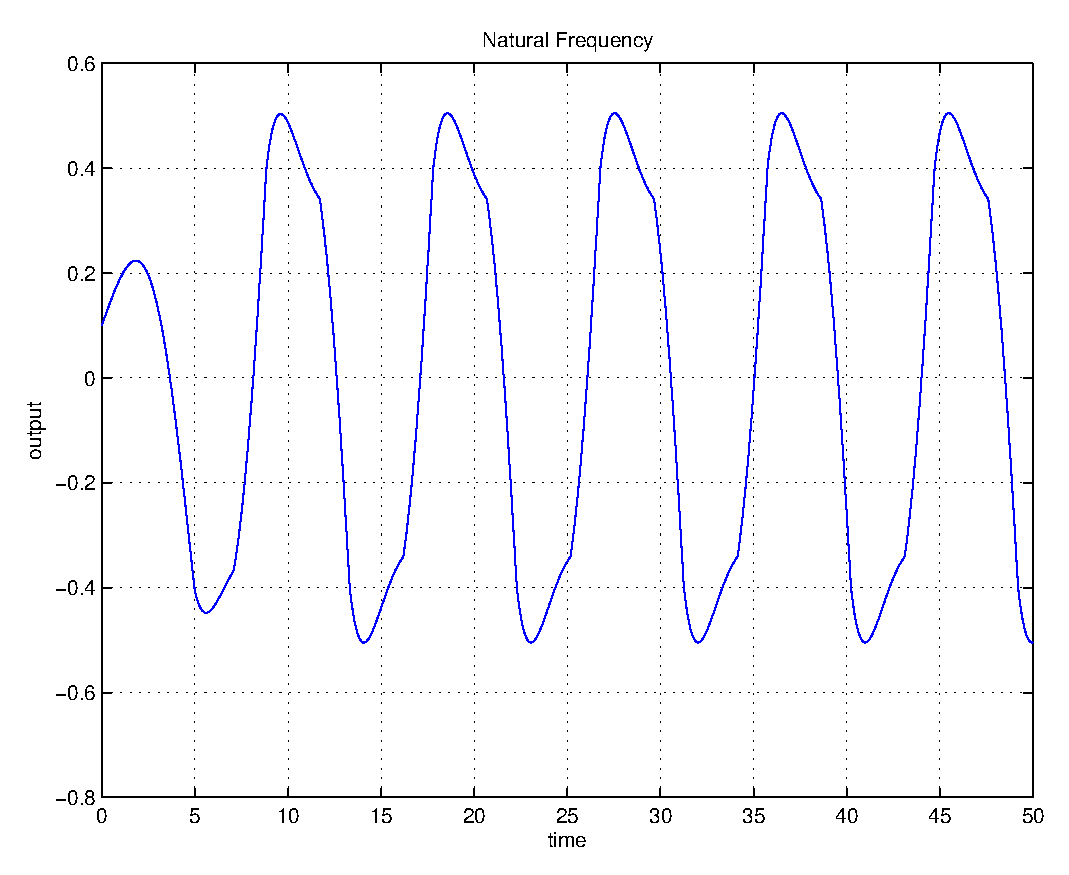
\includegraphics[width=0.5\textwidth]{oscillation}
\caption{Natural Oscillation}
\label{fig:natural-oscillation}
\end{center}
\end{figure}





Matsuoka is adaptive; entrainment can happen when it is coupled with different oscillators. 
Figure~\ref{fig:entraint-oscillation} shows the entrainment oscillation,where  Matsuoka oscillator synchronises with the input signal.
\begin{figure}[h]
\begin{center}
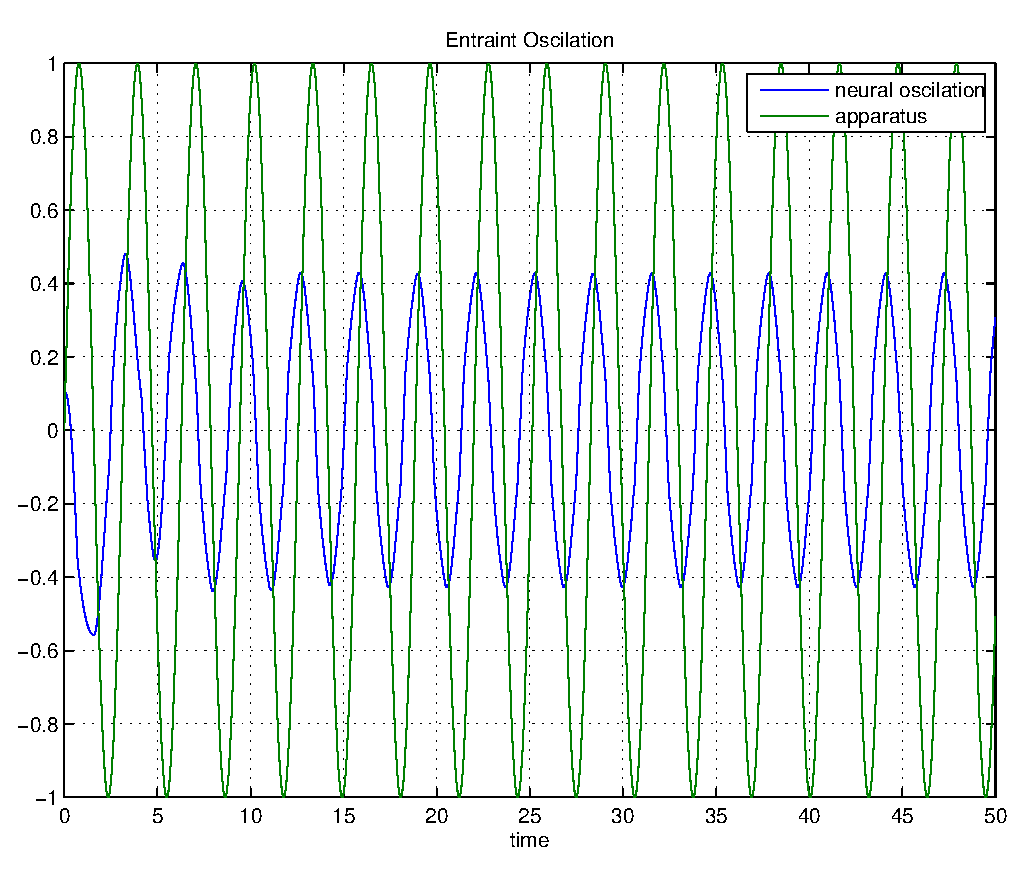
\includegraphics[width=0.5\textwidth]{entraint_oscilation}
\caption{Entrainment Oscillation}
\label{fig:entraint-oscillation}
\end{center}
\end{figure}

Because of the non-linear properties, its behaviour has not been completely understood. 
\citet{Matsuoka1987} analysed the adaptive properties by investigating the location of the roots of the characteristic equation. 
\citet{Williamson1998} analysed the properties in frequency domain.
\citet{futakataentrainment} provided a rigid analysis of energy efficiency and stability for some specific examples.
This research study investigates the qualitative property with  empirical methods.

After examining many simulation results, the Matsuoka Oscillator shows three important properties:
\begin{itemize}
\item{Simple Topological Structure.}
The topology structure of a neural oscillator is simple: 
it includes one  attractive limit circle and one fix repellor.
\item{Large Basin of Attraction.}
All the simulations which we carried out converge to the same limited circle.
\item{Fast Converging Speed.}
In most  cases, the flow will converge to the limit circle within one period time.
\end{itemize}


The above features are shown in Figure ~\ref{fig:neuraldiffinit}.




\begin{figure}[h]
\begin{center}
	\subfigure[state plot]
	{
	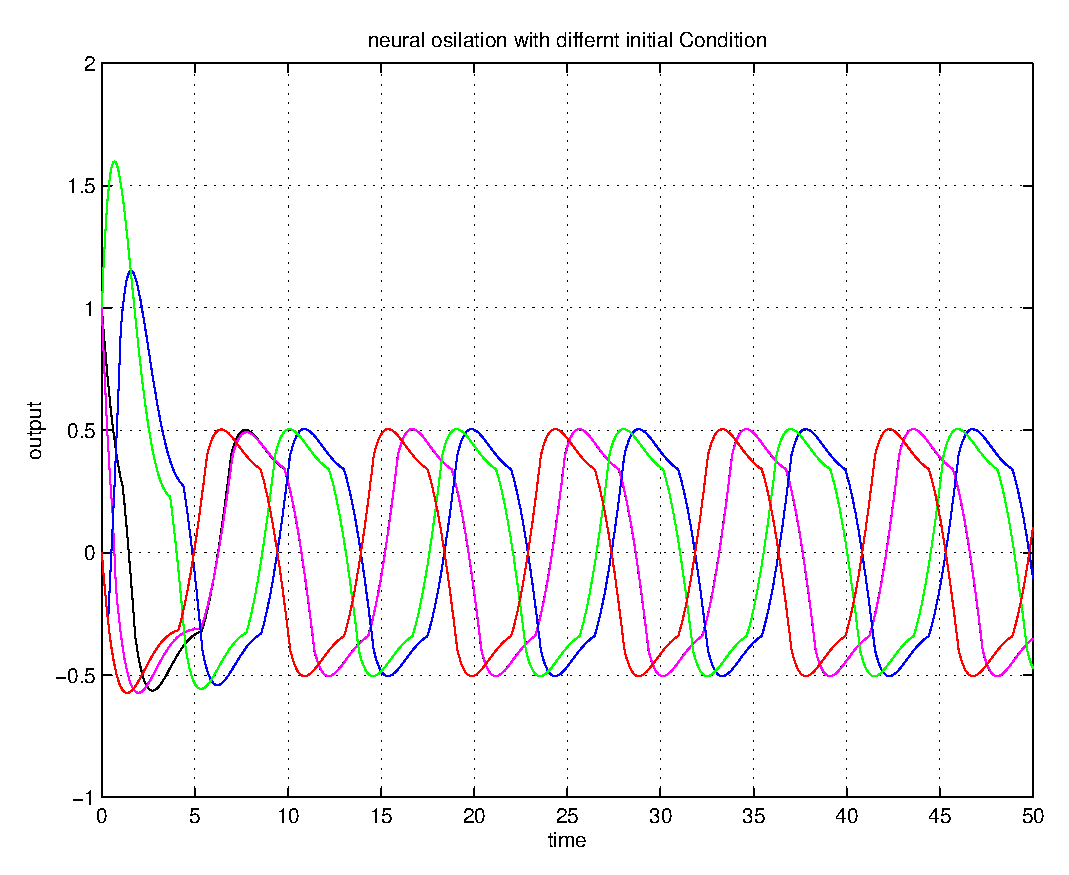
\includegraphics[width=0.45\textwidth]{neural_attraction}
	\label{fig:time_timeAttraction}
	}
	\subfigure[Phase Plane]
	{
	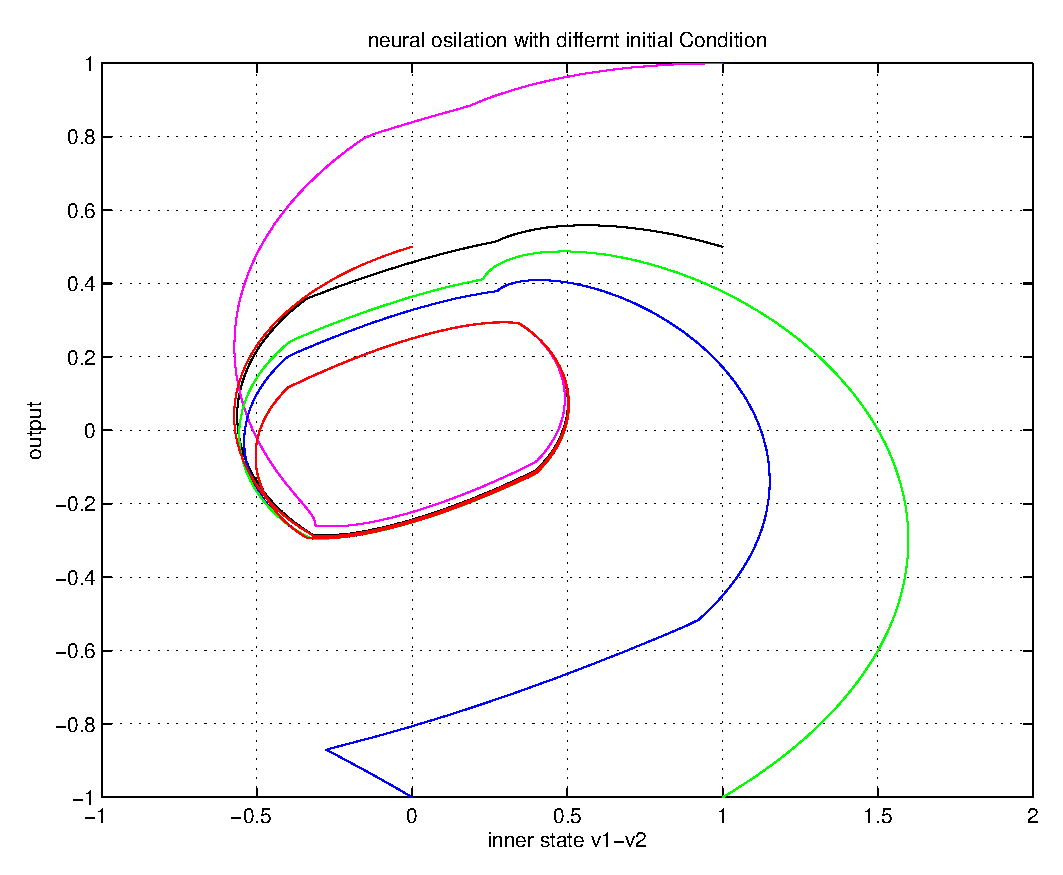
\includegraphics[width=0.45\textwidth]{neural_attraction_phase}
	\label{fig:phase_attraction}
	}
	
\end{center}
\caption{Neural output with different initial positions}
\label{fig:neuraldiffinit}
\end{figure}


 
The large area of basin of attraction means the final behaviour is totally determined by the system parameters. 
The initial conditions will have no effects on the stable oscillation behaviour. 
Matsuota oscillator can be treated as a single input single output(SISO) system.
The output signal is controlled by three system parameters and input signal. 
Equation ~\ref{eq:matsuta} can be reformed as Equation~\ref{eq:simplematsuta}.
\begin{equation}
\uout=S_{[\hin,\hout,\tau]}(\uin)
\label{eq:simplematsuta}
\end{equation}
where $\uin=\sum_{j}h_{j}[w_{j}]$, is the weighted sum of all the input signal.

The converging speed can be seen as a quick recovery ability, which is very valuable for motor control.
When an impulse perturbation happens, it will recover in one period time.


\section{Example:Maintain Ball Bouncing Height}
\label{sec:qualyexample}
The Bouncing Ball system is shown in Figure~\ref{fig:bball}, where a ball is bouncing on a moving paddle.
This system is of simple dynamics, but difficult to control with optimization or \pd\ methods.
\begin{figure}
\begin{center}
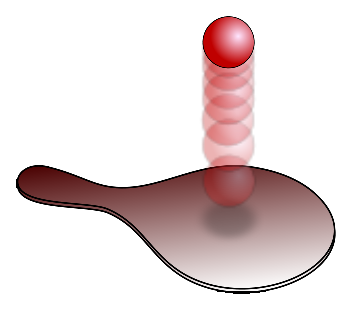
\includegraphics[width=0.5\textwidth]{paddleball}
\end{center}
\caption{The Bouncing Ball System}
\label{fig:bball}
\end{figure}
 
The bouncing ball system captures the complex discontinuous dynamics of body and environment interaction. 
It can be treated as a template model for many motion tasks like jumping, running and ball playing.
This example demonstrates how limit cycle arises through entrainment.
 
\subsection*{Dynamics}
The bouncing ball system is of hybrid dynamic, which involves two phases.
\begin{itemize}
\HiItem{The Continuous Flying Phase:}
When the ball is flying, it is only affected by the gravity.
\HiItem{The Discontinuous Strike Phase:}
When the ball hits the paddle, the speed of the ball is changed instantly.
\end{itemize}
The natural dynamics of bouncing ball system are described by  Equation~\ref{eq:bbeq}.
\begin{align}
\ddot{q}_{ball}&=-\gv &\mathrm{if}\,\,q_{ball} &> q_{paddle}\,\,\mathrm{(free\,\,flying)} \nonumber\\
\dot{q}^{+}_{\mathrm{ball}} - \dot{q}^{+}_{\mathrm{paddle}} &=  \epsilon(\dot{q}^{-}_{\mathrm{ball}} - \dot{q}^{-}_{\mathrm{paddle}})&\mathrm{if}\,\,q_{ball} &\leq {q_{paddle}}\,\,\mathrm{(paddle\,\,strike)}
\label{eq:bbeq}
\end{align}
where $\ddot{q}_{ball}$ is the acceleration,
$\gv$ is the gravity,
$q_{ball},q_{paddle}$ are the positions of the ball and paddle,
$\dot{q}^{+}_{ball,paddle}$ are the speed after a paddle strike and $\dot{q}^{-}_{ball,paddle}$ are the speed before the strike,
$\epsilon$ is collision coefficient $-1 < \epsilon <0$.

Figure~\ref{fig:bborg} shows  plots of the system. 
After each strike, the ball will bounce with a smaller height. 




\begin{figure}[h]
\begin{center}
	\subfigure[state plot]
	{
	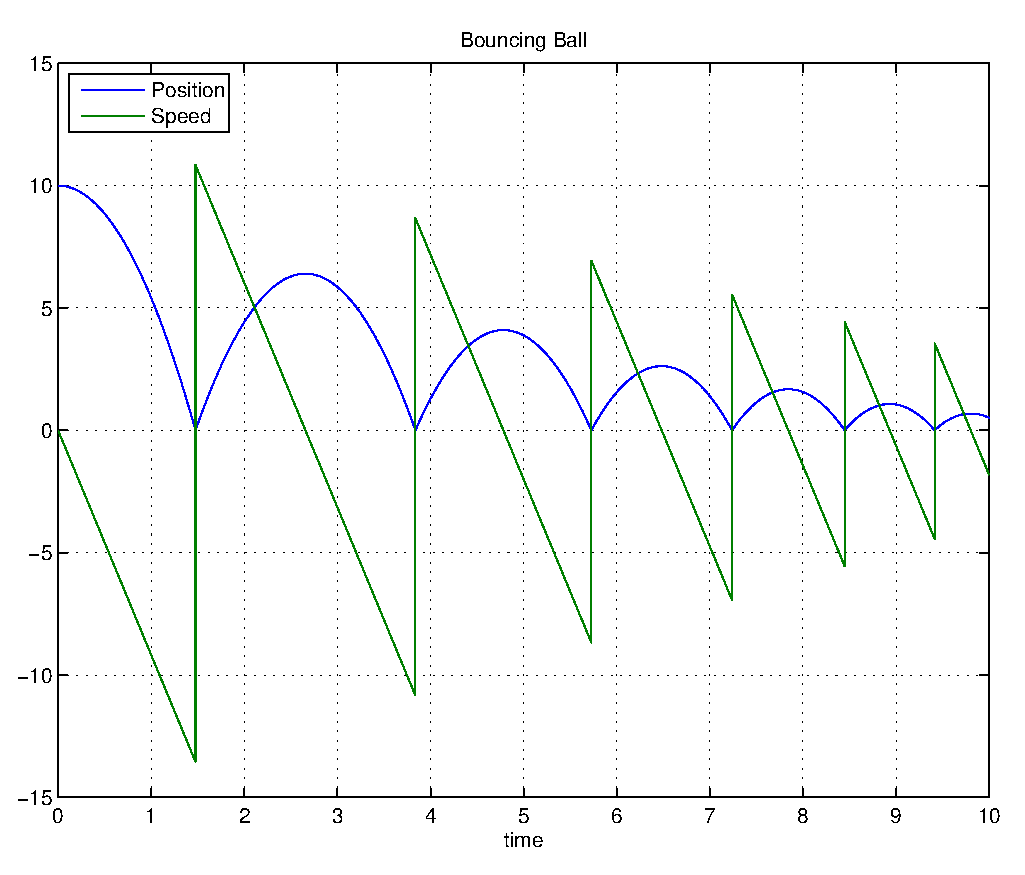
\includegraphics[width=0.45\textwidth]{bouncing_ball}
	\label{fig:bb}
	}
	\subfigure[Phase Plane]
	{
	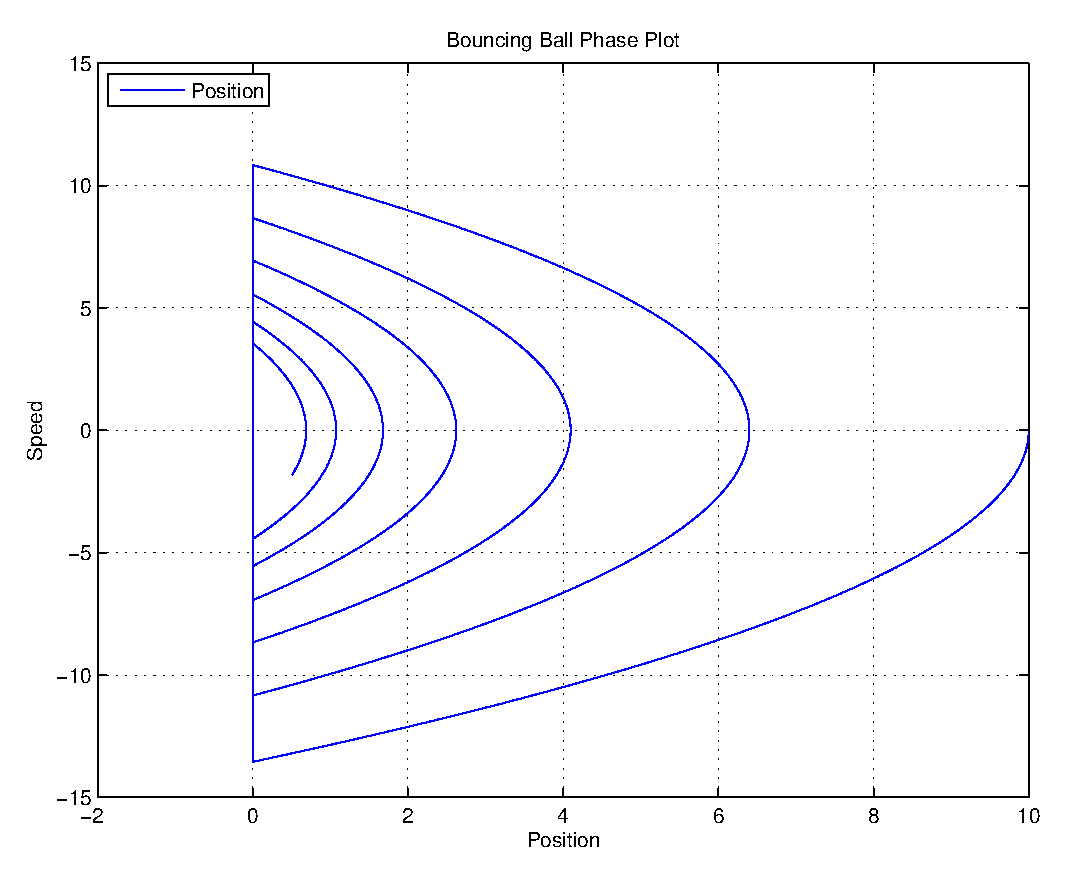
\includegraphics[width=0.45\textwidth]{bouncing_ball_phaseplot}
	\label{fig:bbp}
	}
	
\end{center}
\caption{Original Bouncing Ball System}
\label{fig:bborg}
\end{figure}



\subsection*{Emergence of Limit Cycle}
The  bouncing ball system has only one fixed point attractor and its basin of attraction covers the whole phase space.
However, its behaviour is near periodic.
Or alternatively, it can be seen as a bifurcation of a limit cycle.
Neural Oscillator can be applied to recover the limit cycle through entrainment.
The input of the neural oscillator is the velocity $\uin=\qd_{ball}$, the output drives the paddle position $q_{paddle}=\uout$.
If dropped from different positions, the ball will maintain its bouncing at the height of $5$ units after several strike,
as shown in Figure~\ref{fig:bb_attractive_circle}.

\begin{figure}[h]
\begin{center}
	\subfigure[State Plot]
	{
	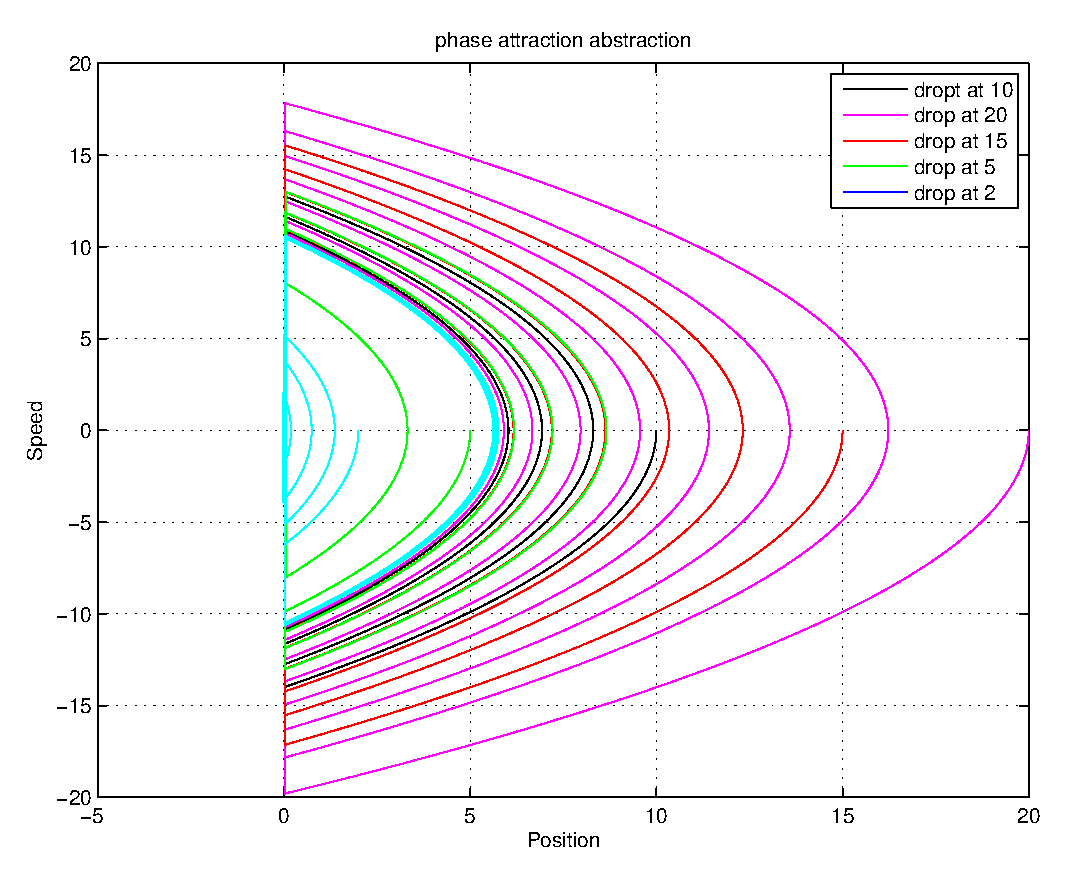
\includegraphics[width=0.45\textwidth]{bb_ms_os_attraction_phase}
	\label{fig:bb_attractive_entraint}
	}
	\subfigure[Phase Plane]
	{
	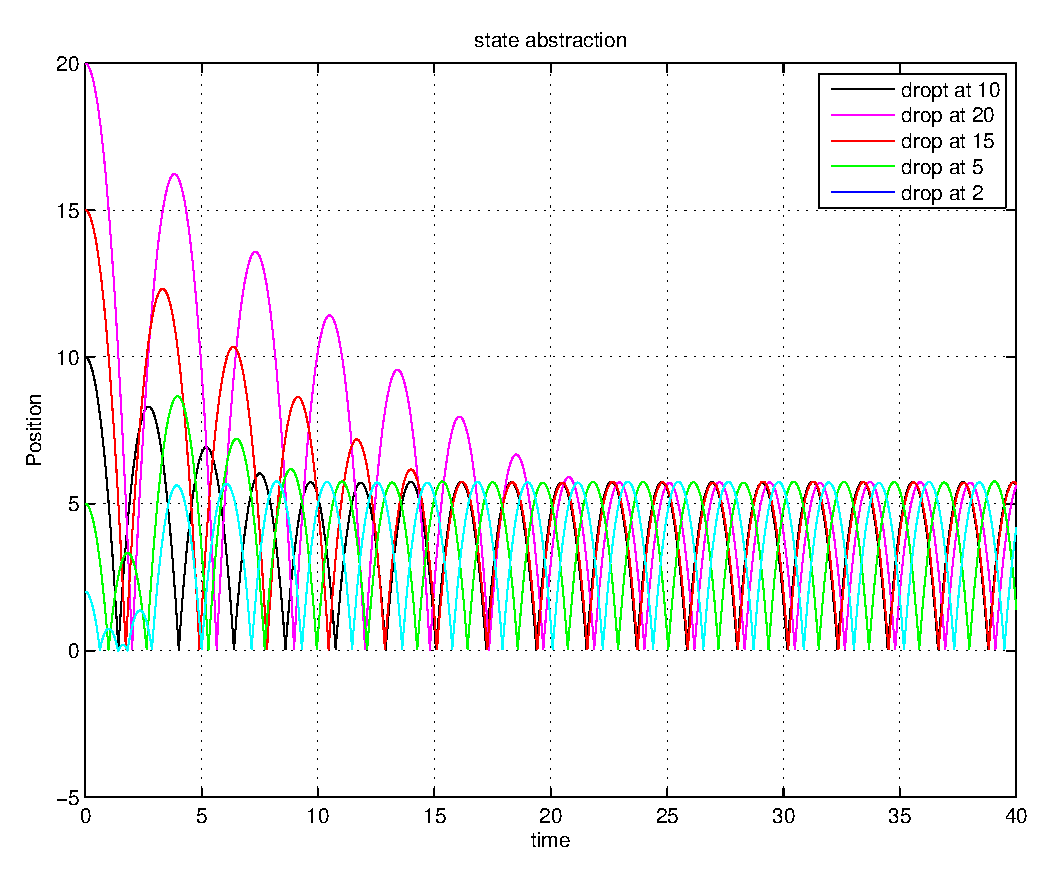
\includegraphics[width=0.45\textwidth]{bb_ms_os_StateTimeAttraction}
	\label{fig:bb_attractive_entraint_time}
	}
	
\end{center}
\caption{The Attractive Limited Circle of the Coupled Bouncing Ball System}
\label{fig:bb_attractive_circle}
\end{figure}

